\begin{frame}{Problem: Over-fitting in a Neural Network}
    \begin{figure}
        \centering
        \href{https://algotrading101.com/learn/what-is-overfitting-in-trading/}{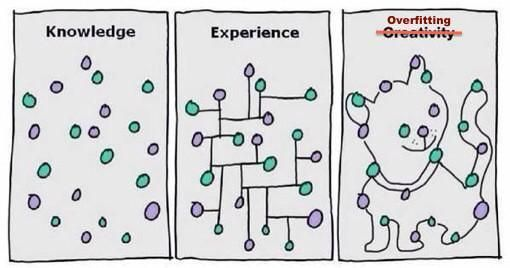
\includegraphics[width=0.8\textwidth]{Figs/section_4/image.png}}
    \end{figure}
\end{frame}

\begin{frame}{Solution 1: L1/L2 regularization}
    \begin{itemize}
        \item just like a classic regularizer
        \item sum the regularizer term for every layer weight
    \end{itemize}
    \vspace{0.2\textheight}
    \begin{equation*}
        \mathlarger{\mathlarger{\mathlarger{
        L = \frac{1}{N} \sum_{i=1}^{N} L(\phi(x_i), y_i) + \lambda \sum_{i,j,k} R(W_{j,k}^{(i)})
        }}}
    \end{equation*}
\end{frame}
\begin{frame}{Solution 1: L1/L2 regularization}
    \begin{itemize}
        \item review
    \end{itemize}
    \vspace{0.1\textheight}
    \begin{equation*}
        \mathlarger{\mathlarger{\mathlarger{
            L1: R(w) = \vert w\vert
        }}}
    \end{equation*}
    \begin{equation*}
        \mathlarger{\mathlarger{\mathlarger{
            L2: R(w) = w^2
        }}}
    \end{equation*}
    \begin{itemize}
        \item you can also combine the two different regularizers (Elastic net)
    \end{itemize}
    \begin{equation*}
        \mathlarger{\mathlarger{\mathlarger{
        R(w) = \beta w^2 + \vert w\vert
        }}}
    \end{equation*}
\end{frame}

\begin{frame}{Solution 2: Early Stopping}
    \begin{itemize}
        \item Stop learning when the validation error is Minimum
    \end{itemize}
    \begin{figure}[H]
	\centering
        \href{https://medium.com/analytics-vidhya/early-stopping-with-pytorch-to-restrain-your-model-from-overfitting-dce6de4081c5}{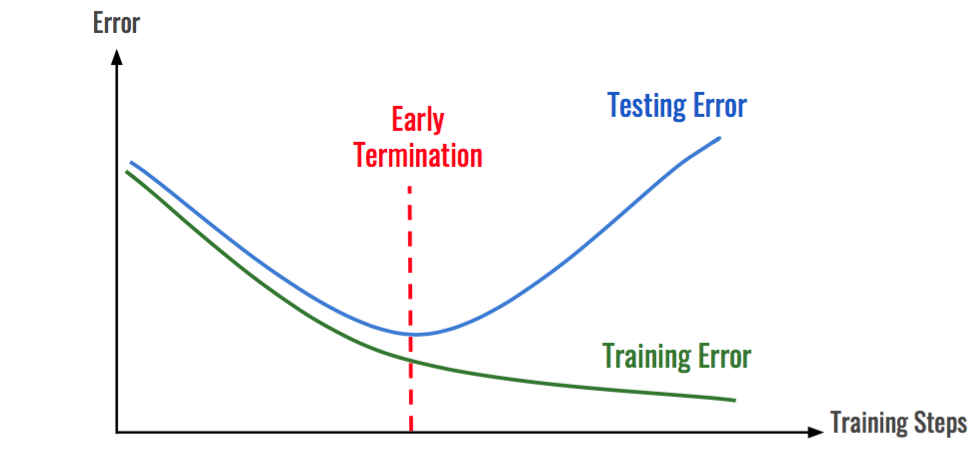
\includegraphics[width=0.8\textwidth]{Figs/Early Stopping.png}}
    \end{figure}
\end{frame}

\begin{frame}{Solution 3: Dropout}
    
\end{frame}

\begin{frame}{Problem: Vanishing/Exploding Gradients}
    
\end{frame}

\begin{frame}{Solution: Batch Norm layer}
    
\end{frame}

% //////////////////
\begin{frame}{Regularization: Dropout}
\begin{itemize}
	\item Randomly set some of neurons to zero in forward pass.
\end{itemize}
\begin{figure}[H]
\centering
\begin{subfigure}[b]{0.3\textwidth}
	\centering
	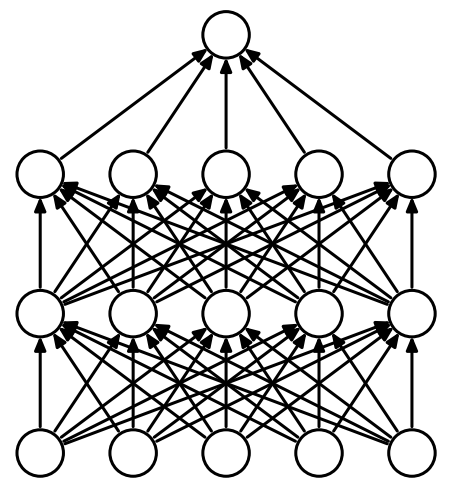
\includegraphics[width=\textwidth]{Figs/Dropout-before.png}
	\caption{Without using dropout}
	\label{fig:Dropout-before}
\end{subfigure}
\begin{subfigure}[b]{0.3\textwidth}
	\centering
	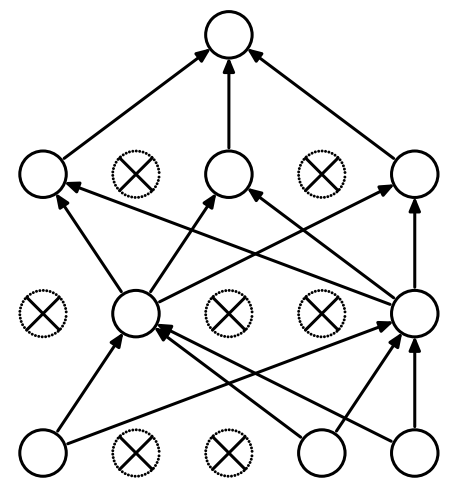
\includegraphics[width=\textwidth]{Figs/Dropout-after.png}
	\caption{After using dropout.}
	\label{fig:Dropout-after}
\end{subfigure}
\caption{Behavior of dropout at training time. \href{https://www.cs.toronto.edu/~hinton/absps/JMLRdropout.pdf}{Source}}
\end{figure}
\end{frame}

\begin{frame}{Regularization: Dropout}
\begin{clomuns}
\begin{column}{0.4\textwidth}
\centering
\begin{figure}[H]
	\centering
	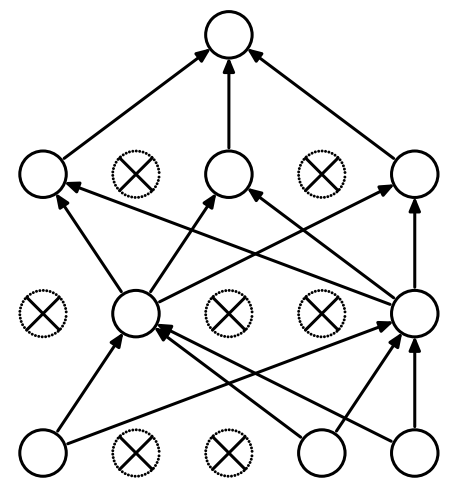
\includegraphics[width=0.9\textwidth]{Figs/Dropout-after.png}
	\caption{\href{https://www.cs.toronto.edu/~hinton/absps/JMLRdropout.pdf}{Source}}
\end{figure}
\end{column}
\begin{column}{0.4\textwidth}
\centering
\begin{itemize}
	\item Dropout:
	\begin{itemize}
		\item Prevents co-adaptation of features (forces network to have redundant representations).
		\item Can be considered a large ensemble of models sharing parameters.
	\end{itemize}
\end{itemize}
\end{column}
\end{clomuns}
% \noindent\begin{minipage}{0.4\textwidth}
% \begin{figure}[H]
% 	\centering
% 	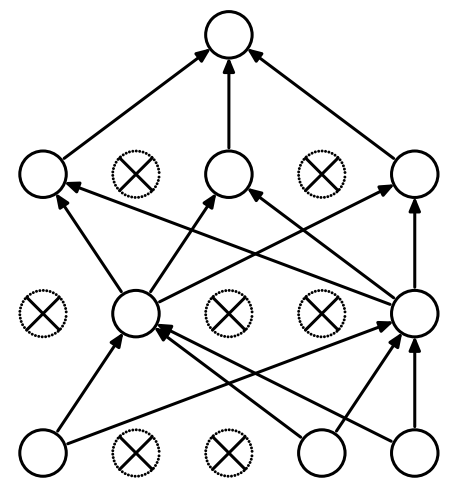
\includegraphics[width=\textwidth]{Figs/Dropout-after.png}
% 	\caption{\href{https://www.cs.toronto.edu/~hinton/absps/JMLRdropout.pdf}{Source}}
% \end{figure}
% \end{minipage}
% \noindent\begin{minipage}{0.4\textwidth}
% \begin{itemize}
% 	\item Dropout:
% 	\begin{itemize}
% 		\item Prevents co-adaptation of features (forces network to have redundant representations).
% 		\item Can be considered a large ensemble of models sharing parameters.
% 	\end{itemize}
% \end{itemize}
% \end{minipage}
\end{frame}

\begin{frame}{Dropout: Test Time}
\begin{itemize}
\item Dropout makes output of network random!
\begin{center}
\begin{tabular}{l@{\hspace{0.25\textwidth}}l}
&$z$: random mask\\
$y = f_W(x, z)$
& $x$: input of the layer\\
& $y$: output of the layer\\
\end{tabular}
\end{center}
\item We want to "average out" the randomness at test time:
\begin{equation*}
y=f(x)=\mathbb{E}_z[f(x, z)] = \int p(z)f(x, z)dz
\end{equation*}

\item Can we calculate the integral exactly?\\
\pause
\item We need to approximate the integral.
\end{itemize}
\end{frame}

\begin{frame}{Dropout: Test Time}
\begin{itemize}
	\item At test time neurons are always present and its output is multiplied by dropout probability:
\end{itemize}
\begin{figure}[H]
	\centering
	\begin{subfigure}[b]{0.3\textwidth}
		\centering
		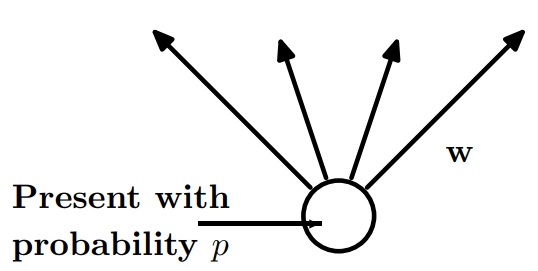
\includegraphics[width=\textwidth]{Figs/dropout-test time-before.png}
		\caption{Without using dropout}
		\label{fig:dropout-test time-before}
	\end{subfigure}
	\begin{subfigure}[b]{0.3\textwidth}
		\centering
		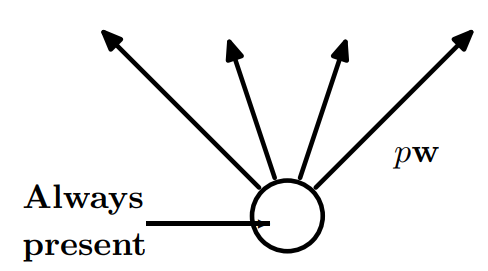
\includegraphics[width=\textwidth]{Figs/dropout-test time-after.png}
		\caption{After using dropout.}
		\label{fig:dropout-test time-after}
	\end{subfigure}
	\caption{Behavior of dropout at test time. \href{https://www.cs.toronto.edu/~hinton/absps/JMLRdropout.pdf}{Source}}
\end{figure}
\end{frame}


\begin{frame}{Regularization: Adding Noise}
\begin{itemize}
\item We've seen a common approach for regularization thus far:
\begin{itemize}
	\item \textbf{Training}: Add some kind of randomness ($z$) : $$y = f_W(x, z)$$
	\item \textbf{Testing}: Average out the randomness: $$y=f(x)=\mathbb{E}_z[f(x, z)] = \int p(z)f(x, z)dz$$
\end{itemize}
\pause
\item Adding noise is another way to prevent a neural network from overfitting on the training data.
In every iteration, a random noise is added to the outputs of the layer, preventing consequent layers from co-adapting too much to the outputs of this layer.
\end{itemize}
\end{frame}

\begin{frame}{Batch Normalization}
\begin{tabular}{l l}
Input: $x: N\times D$ & Learnable Parameters: $\gamma, \beta: D$\\
Output: $y: N\times D$ & Intermediates: $\mu, \sigma: D$, $\hat{x}: N \times D$
\end{tabular}
\begin{align*}
\mu_j &= \textup{(Running) average of values seen during training}\\
\sigma^2_j &= \textup{(Running) average of values seen during training}\\
\hat{x}_{i, j} &= \frac{x_{i, j} - \mu_j}{\sqrt{\sigma^2_j + \epsilon}}\\
y_{i,j} &= \gamma_j \hat{x}_{i, j} + \beta_j
\end{align*}
\end{frame}

\begin{frame}{Batch Normalization}
\begin{itemize}
\item Batch normalization is done along with \textbf{C} axis in convolutional networks:
\begin{figure}
	\centering
	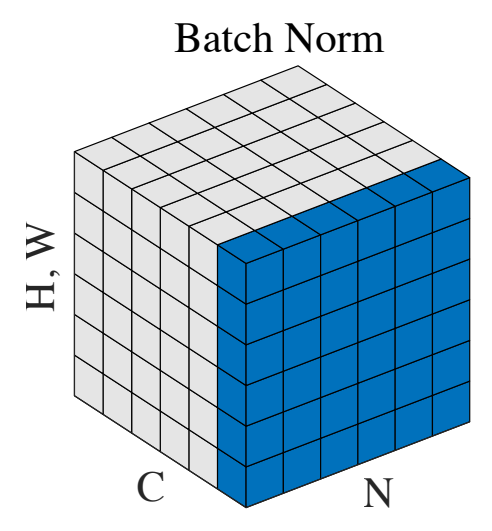
\includegraphics[width=0.3\textwidth]{Figs/batch normalization for cnn.png}
	\caption{Batch normalization in CNNs \href{https://arxiv.org/pdf/1803.08494.pdf}{Source}.}
	\label{fig:batch normalization for cnn}
\end{figure}
\begin{itemize}
\item BN for FCNs: $x, y: N\times D \rightarrow \mu, \sigma, \gamma, \beta: 1\times D$
\item BN for CNNs: $x, y: N\times C \times H \times W \rightarrow \mu, \sigma, \gamma, \beta: 1\times C \times 1 \times 1$
\item In both cases: $y = \gamma (x - \mu) / \sigma + \beta$
\end{itemize}
\end{itemize}

\end{frame}